\documentclass{beamer}

\mode<presentation> {

% The Beamer class comes with a number of default slide themes
% which change the colors and layouts of slides. Below this is a list
% of all the themes, uncomment each in turn to see what they look like.

%\usetheme{default}
%\usetheme{AnnArbor}
%\usetheme{Antibes}
%\usetheme{Bergen}
%\usetheme{Berkeley}
%\usetheme{Berlin}
%\usetheme{Boadilla}
%\usetheme{CambridgeUS}
%\usetheme{Copenhagen}
%\usetheme{Darmstadt}
%\usetheme{Dresden}
%\usetheme{Frankfurt}
%\usetheme{Goettingen}
%\usetheme{Hannover}
%\usetheme{Ilmenau}
%\usetheme{JuanLesPins}
%\usetheme{Luebeck}
\usetheme{Madrid}
%\usetheme{Malmoe}
%\usetheme{Marburg}
%\usetheme{Montpellier}
%\usetheme{PaloAlto}
%\usetheme{Pittsburgh}
%\usetheme{Rochester}
%\usetheme{Singapore}
%\usetheme{Szeged}
%\usetheme{Warsaw}

% As well as themes, the Beamer class has a number of color themes
% for any slide theme. Uncomment each of these in turn to see how it
% changes the colors of your current slide theme.

%\usecolortheme{albatross}
%\usecolortheme{beaver}
%\usecolortheme{beetle}
%\usecolortheme{crane}
%\usecolortheme{dolphin}
%\usecolortheme{dove}
%\usecolortheme{fly}
%\usecolortheme{lily}
%\usecolortheme{orchid}
%\usecolortheme{rose}
%\usecolortheme{seagull}
%\usecolortheme{seahorse}
%\usecolortheme{whale}
%\usecolortheme{wolverine}

%\setbeamertemplate{footline} % To remove the footer line in all slides uncomment this line
%\setbeamertemplate{footline}[page number] % To replace the footer line in all slides with a simple slide count uncomment this line

%\setbeamertemplate{navigation symbols}{} % To remove the navigation symbols from the bottom of all slides uncomment this line
}

\usepackage{graphicx} % Allows including images
\usepackage{booktabs} % Allows the use of \toprule, \midrule and \bottomrule in tables
\usepackage[utf8]{inputenc}

%----------------------------------------------------------------------------------------
%	TITLE PAGE
%----------------------------------------------------------------------------------------

\title[Google Home]{Google Home Final Presentation} % The short title appears at the bottom of every slide, the full title is only on the title page

\author{Mehmet Kardan, Hanna Köb, Mathias Meinschad, Daniel Linter} % Your name
\institute[UCLA] % Your institution as it will appear on the bottom of every slide, may be shorthand to save space
{
University of Innsbruck - SIT \\ % Your institution for the title page
}
\date{\today} % Date, can be changed to a custom date

\begin{document}

\begin{frame}
\titlepage % Print the title page as the first slide
\end{frame}

\begin{frame}
\frametitle{Overview} % Table of contents slide, comment this block out to remove it
\tableofcontents % Throughout your presentation, if you choose to use \section{} and \subsection{} commands, these will automatically be printed on this slide as an overview of your presentation
\end{frame}

%----------------------------------------------------------------------------------------
%	PRESENTATION SLIDES
%----------------------------------------------------------------------------------------

%------------------------------------------------
\section{Overview}

\begin{frame}
\frametitle{Overview}
\begin{center}

\includegraphics[scale=0.35]{pictures/google-home.png} 
\end{center}
\begin{itemize}
\item Founded by Google in 2016
\item Development through Googles developer console and Dialogflow
\item Creating skills pretty easy
\item No programming skills required
\end{itemize}
\end{frame}

\begin{frame}
\frametitle{Device Types \& Traits}
\begin{center}
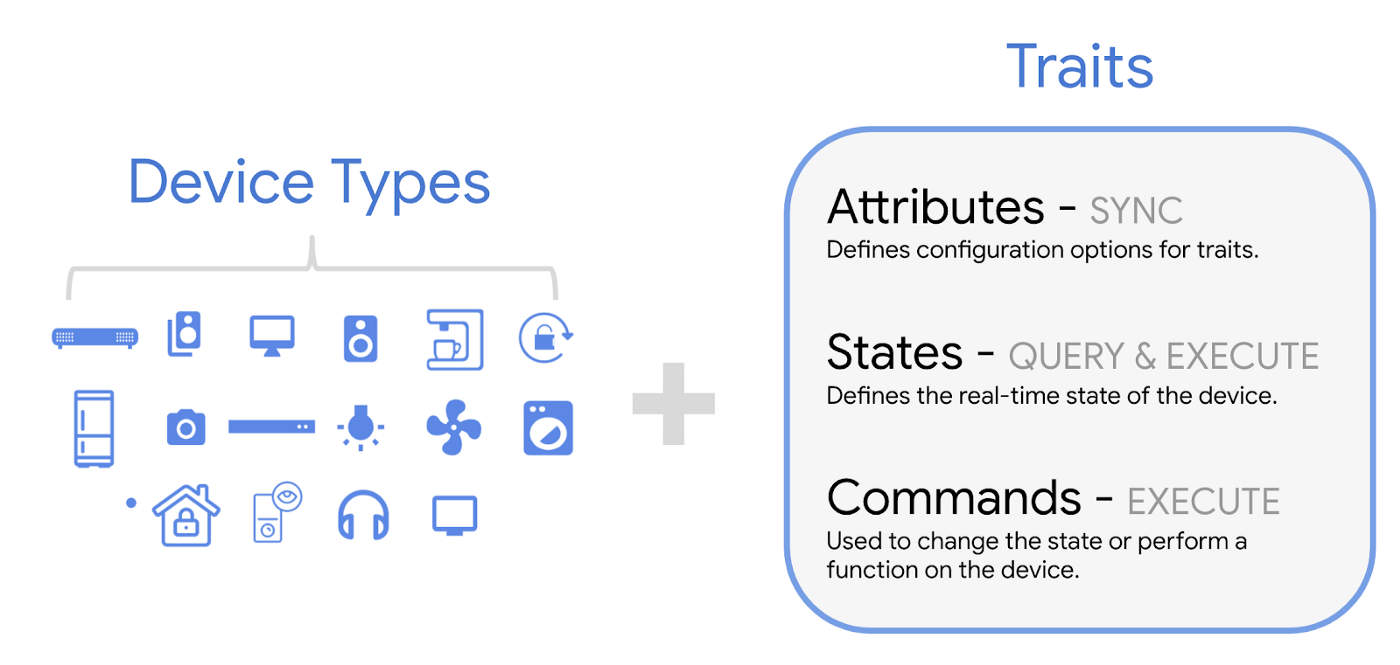
\includegraphics[scale=0.2]{pictures/state_commands.png} 
\end{center}
\begin{itemize}
\item Various device types ( air purifier to yogurt maker )
\item Capabilities of a device $\Rightarrow$ traits
\end{itemize}
\end{frame}

%------------------------------------------------

\section{Execution Path}

\begin{frame}
\frametitle{Execution Path}
\begin{center}
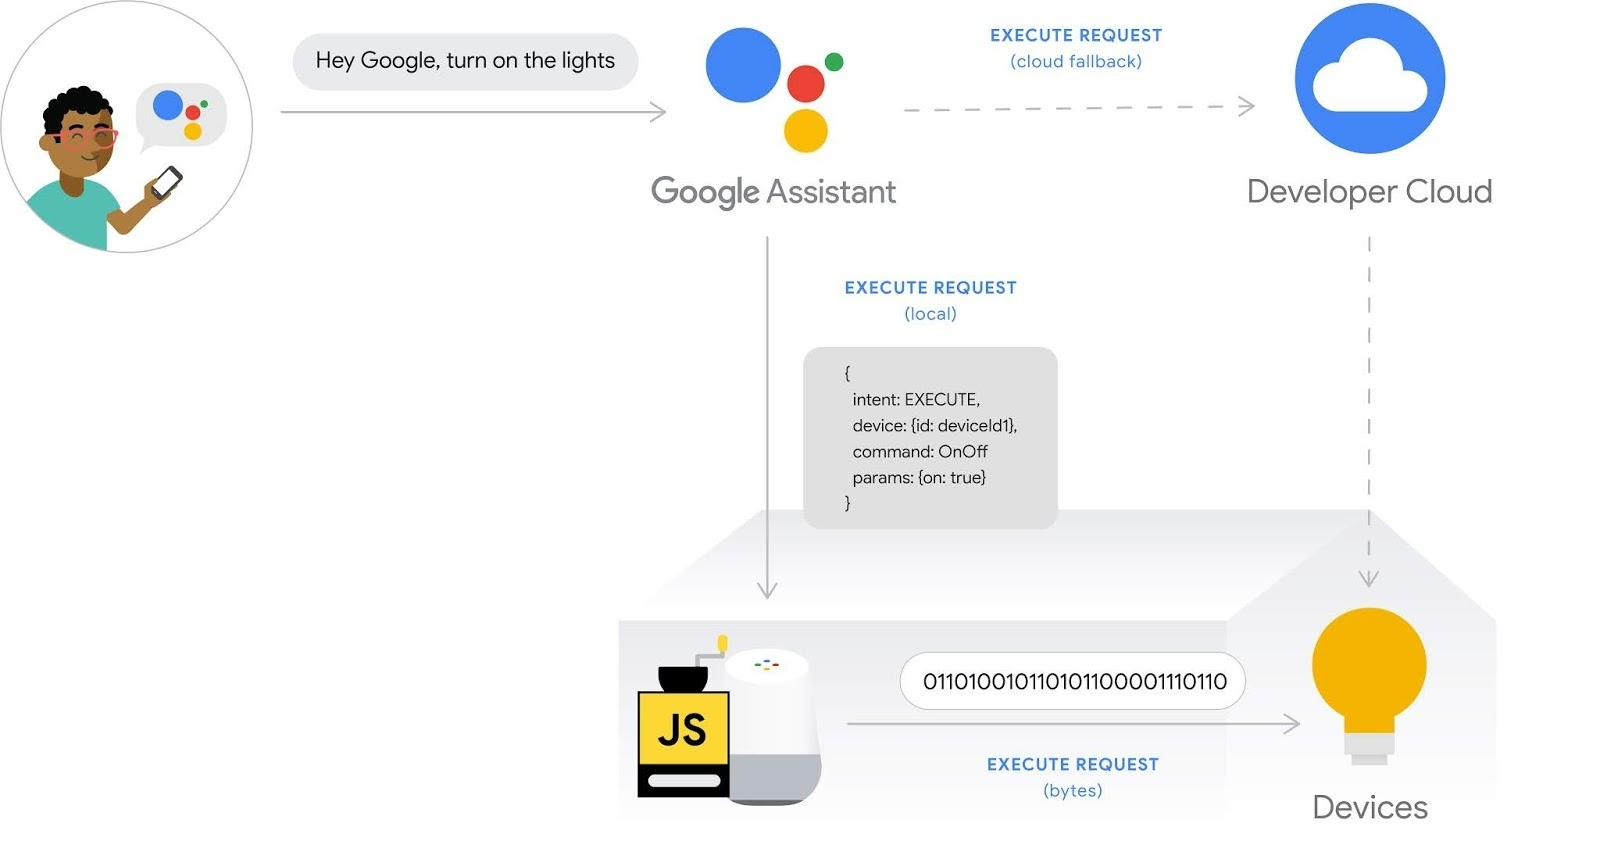
\includegraphics[scale=0.2]{pictures/execution-path.png}
\end{center}
\end{frame}

%------------------------------------------------

\subsection{Intents}

\begin{frame}
\frametitle{Intents}
\begin{center}
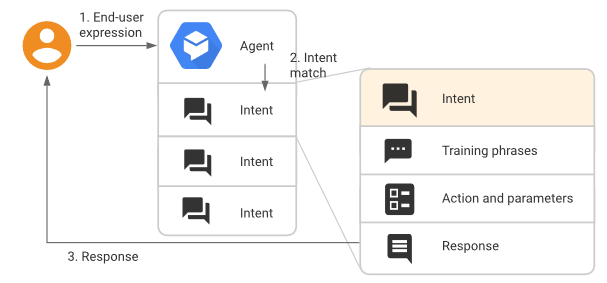
\includegraphics[width=0.8\textwidth]{pictures/intent.png}

\end{center}
\end{frame}

\begin{frame}
\frametitle{Intents cont'd}
\begin{center}
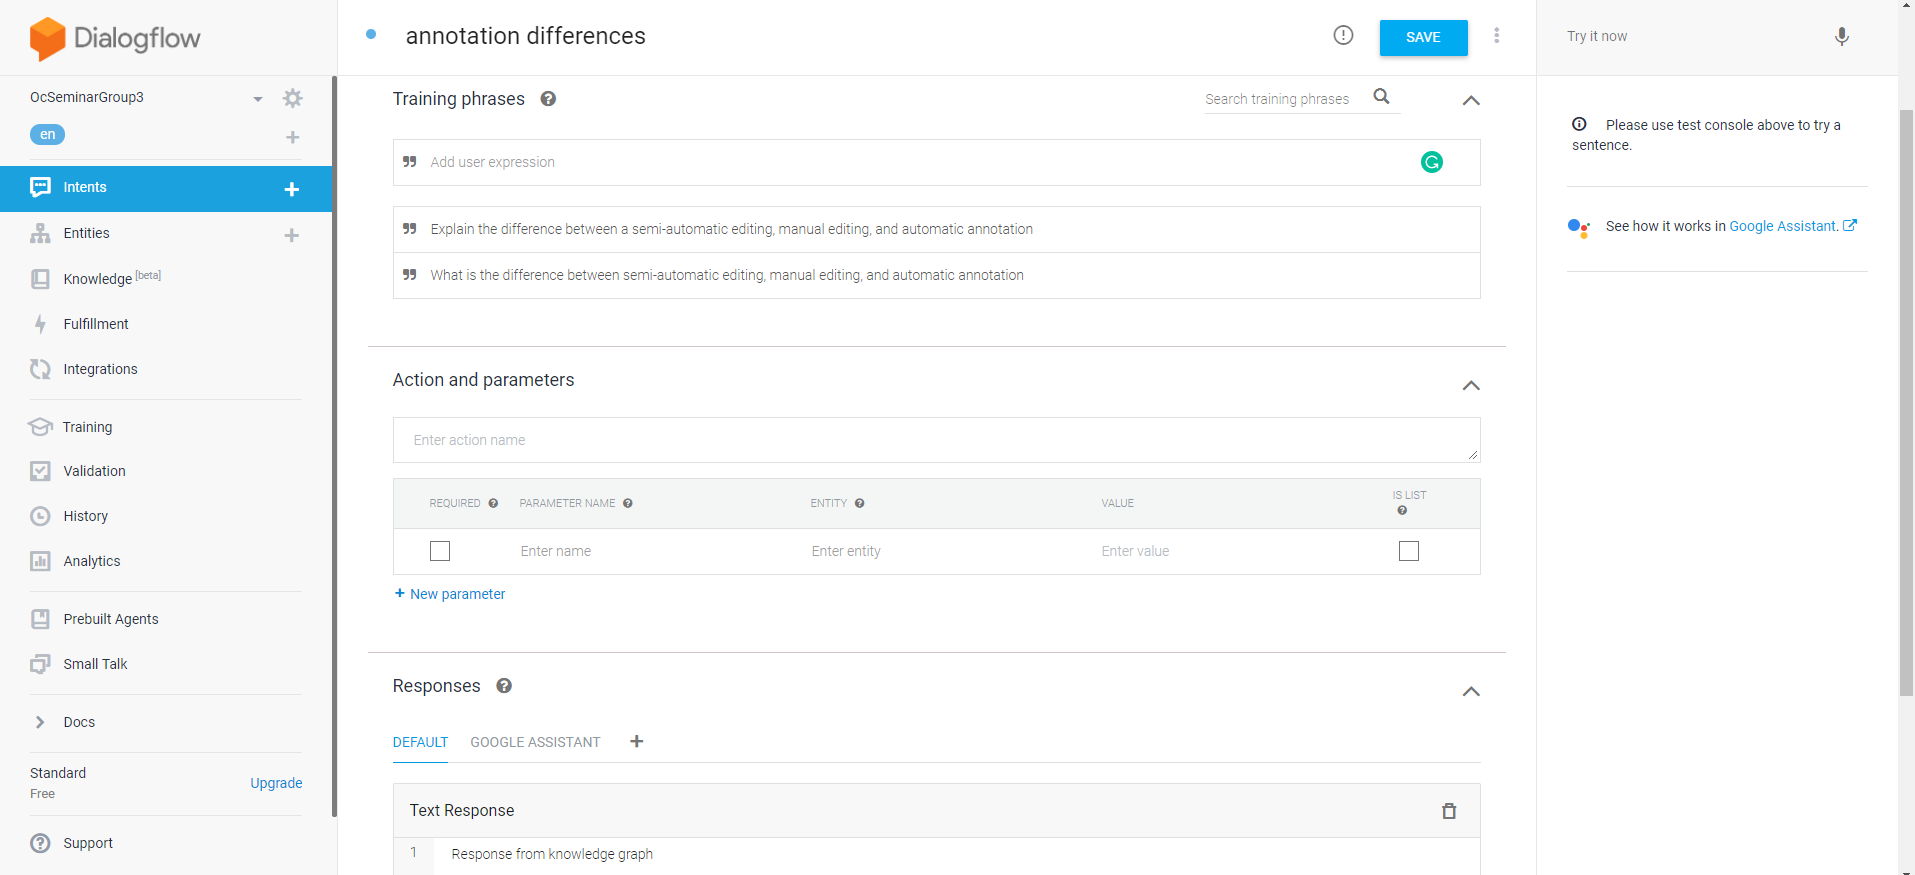
\includegraphics[width=\textwidth]{pictures/intents.png}

\end{center}
\end{frame}

%------------------------------------------------

\subsection{Entities}

\begin{frame}
\frametitle{Entities}
\begin{center}
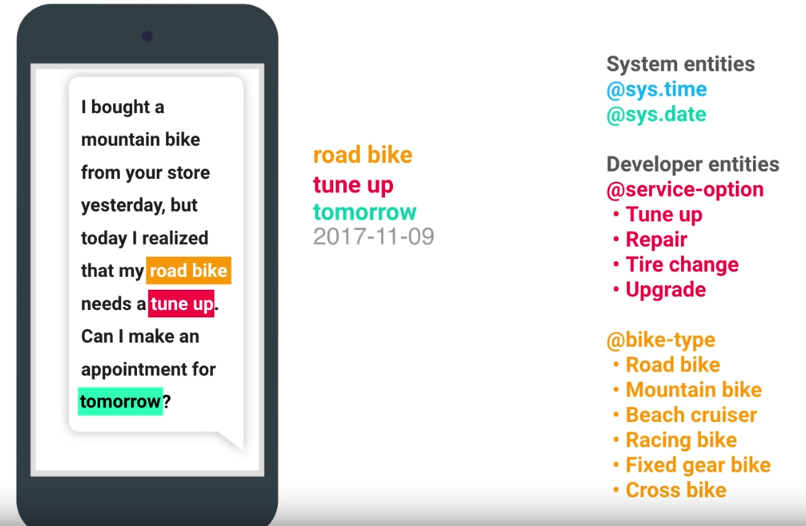
\includegraphics[width=0.8\textwidth]{pictures/entities2.png}
\end{center}
\end{frame}

\begin{frame}
\frametitle{Entities cont'd}
\begin{center}
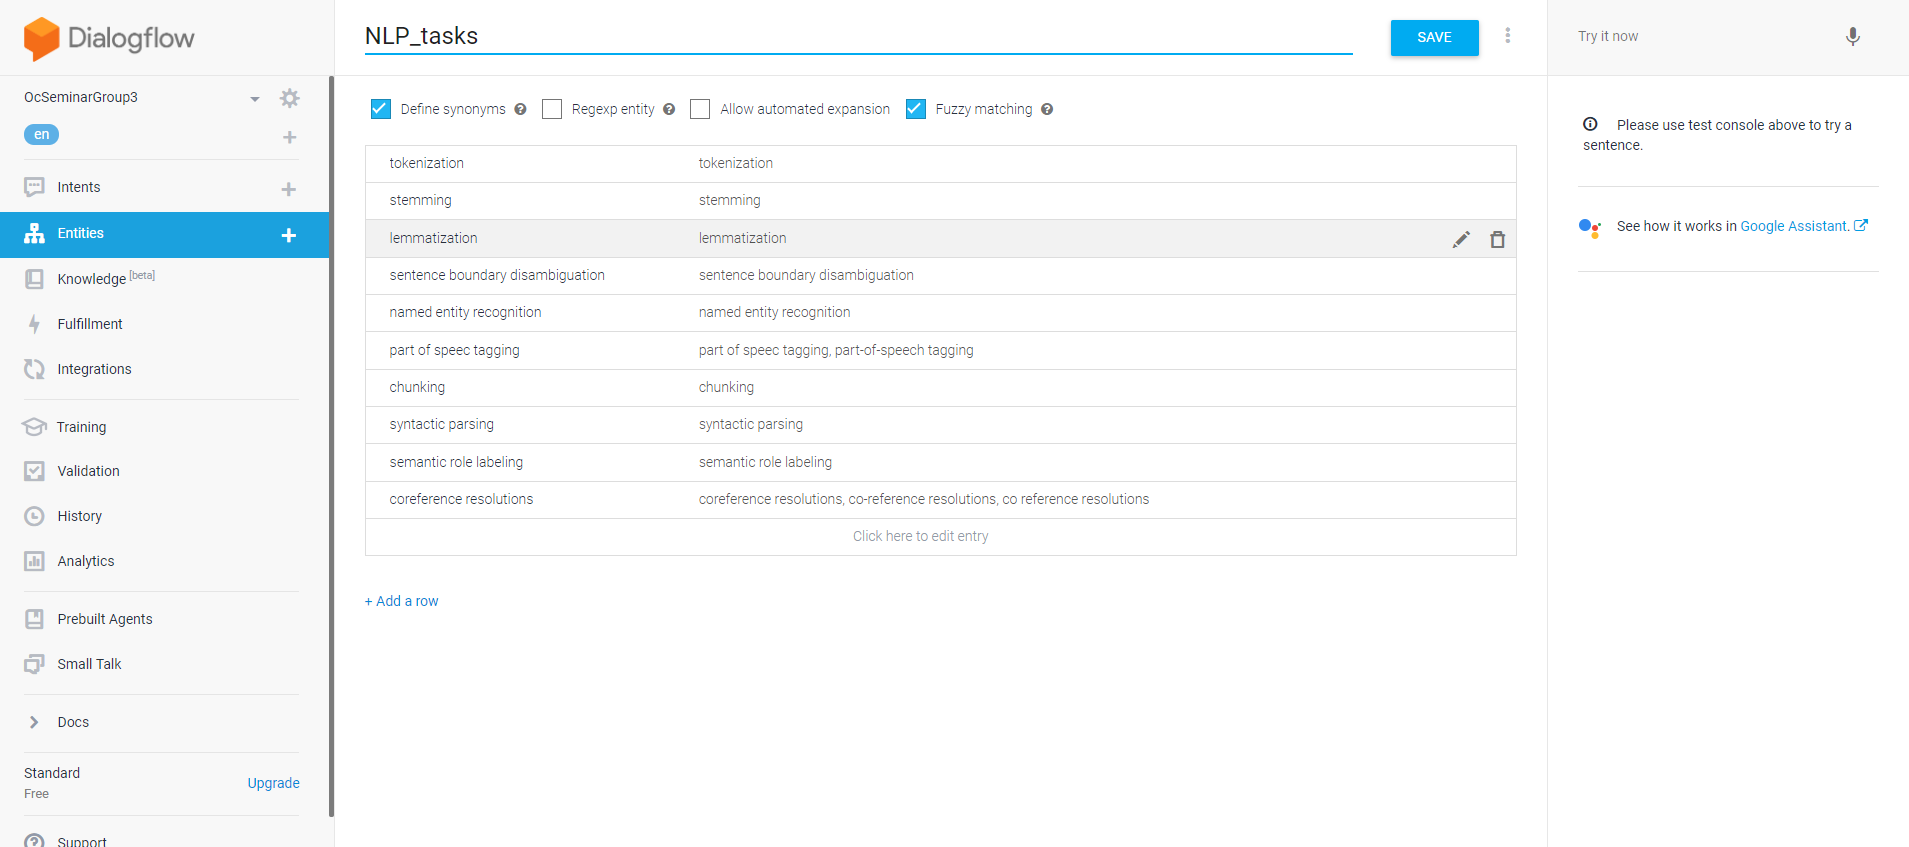
\includegraphics[width=\textwidth]{pictures/entities.png}
\end{center}
\end{frame}

%------------------------------------------------

\subsection{Fulfillment}

\begin{frame}
\frametitle{Fulfillment}
\begin{center}
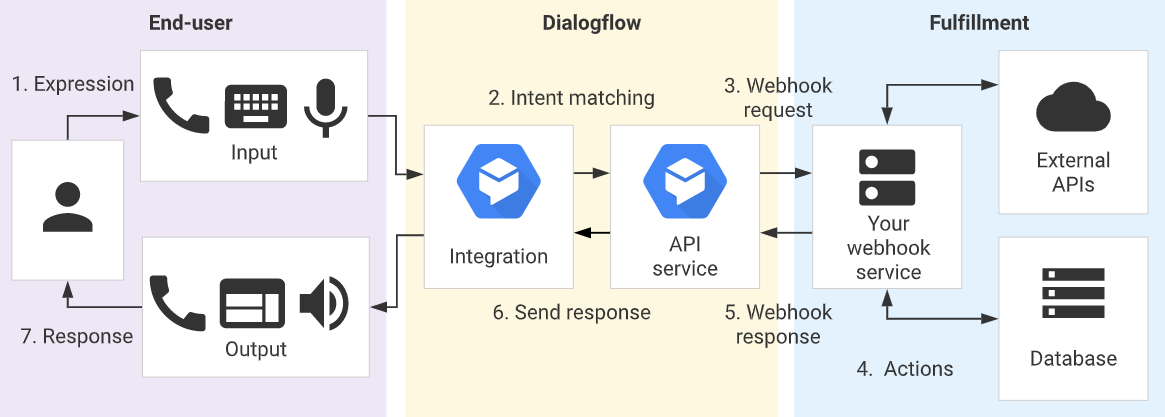
\includegraphics[width=\textwidth]{pictures/fulfillment_flow.png} 
\end{center}
\end{frame}


\begin{frame}
\frametitle{Communication}
\begin{center}
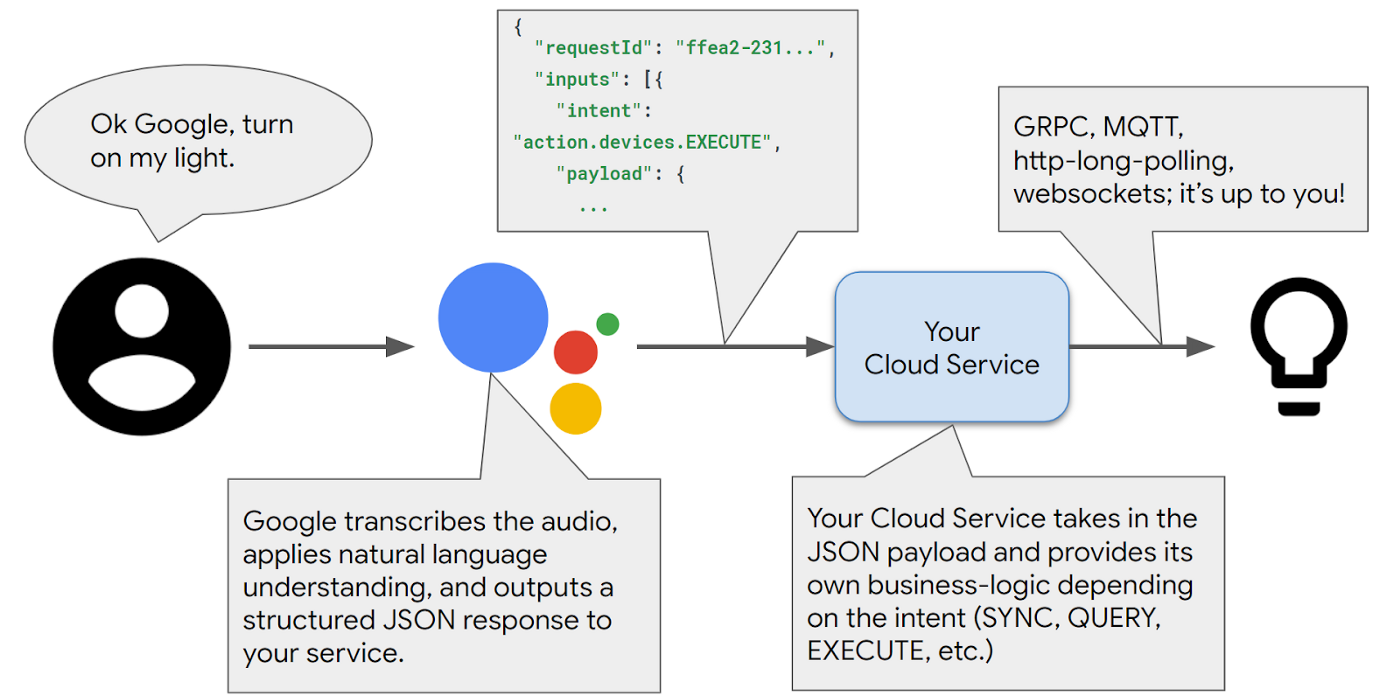
\includegraphics[scale=0.22]{pictures/communication_btw.png}
\end{center}
\end{frame}

%------------------------------------------------

\section{Live Demo}

\begin{frame}
\frametitle{Live Demo}
\begin{center}
{\fontsize{30}{40}\selectfont Live Demo}
\end{center}
\end{frame}

%------------------------------------------------

\begin{frame}
\begin{center}
{\fontsize{30}{40}\selectfont Thank you for your attention!}
\end{center}
\end{frame}

%------------------------------------------------

\end{document} 
